\chapter{Discussion}\label{chap:discussion}

This chapter presents a reflection on both the development process and the final product. It examines how the project evolved in relation to the original goals, highlighting what worked well, what could have been improved, and the challenges encountered along the way. The chapter discusses the choice of technologies, project management practices, and team collaboration. It also evaluates the effectiveness and limitations of the final solution, comparing it with existing alternatives and identifying unexpected findings. Broader considerations, such as sustainability and the role of AI in the project, are explored. Finally, the chapter outlines potential directions for future work and improvements to both the product and the project approach.

\section{Process}

This section provides a reflection on the project's development process, covering both planning and execution. It examines how the initial project plan guided the work, the technologies that were selected, and the software development methodology that was followed. The section also evaluates the collaboration within the group, including how communication was handled and how responsibilities were distributed. In addition, it highlights areas where the process could have been improved, and describes how AI tools were used throughout the project to support development, planning, or writing tasks.

\subsection{Project Plan}

Looking back, we were able to follow the project plan for the most part, but there were certain parts that either were moved around to other times or removed entirely for practical reasons. The hardest part when planning was knowing how much time to allocate to each part of the project. There were multiple times where we had either worked faster than expected or had to postpone tasks due to unforeseen issues. \textcolor{orange}{gi noen eksempler på hvordan dette kunne blitt gjort bedre, planning poker? Kanskje ikke like effektivt da man kun er 2 i gruppen siden vi ofte var enige om det meste.}

One of the biggest strengths of our project plan was the structure provided by Scrum and the use of sprints. The plan’s division into eight sprints allowed us to stay focused and iterative, and it gave us frequent opportunities to re-evaluate priorities and progress. However, we found that the sprint content sometimes had to be adjusted mid-way through to accommodate emerging challenges, such as unexpected bugs, delays in data access, or changes in user feedback. Knowing this, the sprint length could potentially have been shorter, e.g., the first few sprints were 1-week then the later ones could have been 2-weeks. 

Our Gantt chart helped define clear milestones, like the MVP, and these helped us stay aligned with deliverables. Nevertheless, actual progress often didn’t align perfectly with the chart. For instance, early on we had a whole sprint for research, data collection and system design. In hindsight we only needed half a sprint for this and therefore we started designing the website which was planned for the next sprint. In later sprints we had planned user tests which kept getting pushed back, and in the end the formal user tests were replaced with feedback from the Product Owner and a presentation of the product for potential stakeholders.

The inclusion of the vacation in the plan was helpful, and having accountability measures, like compensating for delays by using it as a buffer, proved valuable in practice. The group contract and routine rules also helped maintain consistent effort and communication, although there were still minor challenges in balancing workloads week to week.

Another challenge was scope control. As predicted in the risk analysis, there was some pressure to expand the scope with more features or data sources. \textcolor{orange}{f.eks. skrive om at kartet støtter hele norge istedenfor bare gjøvik?}. Regular sprint meetings with our supervisor also played a key role in maintaining focus.

The use of GitHub for both version control and task management via the Kanban board made it easy to track progress and adjust tasks as needed. This complemented the Scrum framework well and allowed us to keep the project transparent and adaptable.

\subsection{Technologies}

This section contains a reflection of the different technologies and tools used throughout the project. We discuss both the client-side and server-side components, as well as supporting tools that contributed to collaboration, version control, and project management. The chosen technologies were selected based on factors such as ease of integration, documentation quality, performance, and our team's familiarity with them, or lack thereof.

\subsubsection{Website}

The chosen technologies for the website, TypeScript, React, and OpenLayers, proved to be well-suited for the project. Although we had little prior experience with these tools, their extensive documentation allowed us to quickly learn them throughout the development process.

While the overall scope of the application is moderate, using TypeScript instead of JavaScript significantly improved type safety and reduced the likelihood of runtime errors. This added confidence during development and helped maintain code quality.

We had limited prior experience with web development, so we cannot directly compare React to building a website without a framework. However, React’s component-based structure made it easy to build and reuse interface elements, which likely made the development process more efficient and maintainable.

\textcolor{orange}{OpenLayers: sammenligne med leaflet her eller tidligere i rapporten?}

\subsubsection{Server}

As described in \autoref{chap:implementation}, we made good use of the advantages of Go (?rewrite). 

\subsubsection{Div ekstra (traggo, github org med kanban, skyhigh)}

\subsection{SDLC Model / SCRUM}

\textcolor{orange}{NOE TEKST}

\subsection{Communication}

\textcolor{orange}{NOE TEKST}

\subsection{Work Allocation}

\textcolor{orange}{blabla}

\autoref{tab:timetrackedbymember} shows the total time of work for each month by the two members.

\begin{table}[h]
    \centering
    \begin{tabular}{c|c|c|c}
        \hline
        \textbf{Month} & \textbf{Bjørnsen} & \textbf{Houmb} & \textbf{Total} \\
        \hline
        January  & 61h 39m  & 62h 58m  & 124h 37m \\
        February & 80h 6m   & 79h 17m  & 159h 24m \\
        March    & 88h 4m   & 88h 20m  & 176h 24m \\
        April    & 99h 40m  & 102h 38m  & 202h 18m \\
        May      &        &        &        \\
        \hline
        Total & & & \\
        \hline
    \end{tabular}
    \caption{Tracked time by month and group member}
    \label{tab:timetrackedbymember}
\end{table}

% Skriv mer om time fordeling, f.eks. hvorfor mer timer i mars enn januar etc.

\autoref{fig:time_tracking_by_type} shows the total time of work for each month by the two members.

% KANSKJE IKKE TA SKJERMBILDE, LAG HELLER CHART MED LATEX f.eks. (pfg-pie).
\begin{figure}[h]
    \centering
    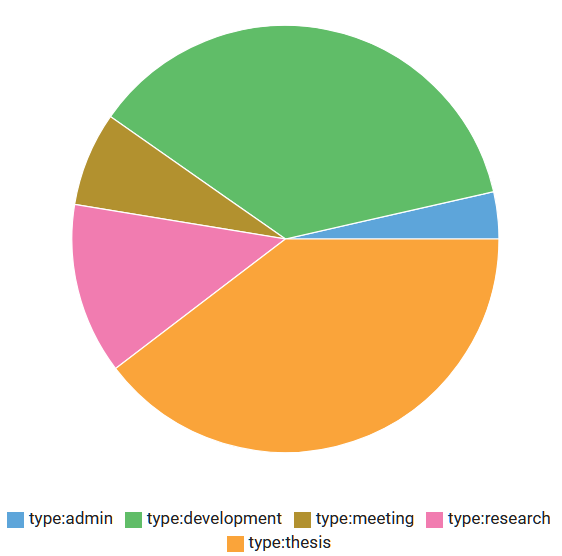
\includegraphics[width=0.5\linewidth]{figures/traggo_pie_chart_by_type.png}
    \caption{Pie chart of time spent in total per work type}
    \label{fig:time_tracking_by_type}
\end{figure}

\textcolor{orange}{GJØR PIECHART HVIT FOR PRINTING}

% SKRIV OM TIDSFORDELING FOR DE FORSKJELLIGE OPPGAVENE (THESIS, DEV, osv.)

\subsection{Improvements}

\textcolor{orange}{Kanskje nevne Universal Design? \\ \\
Hva mente du med improvements her? Vil ikke future work dekke? /e}

\subsection{Use of AI}

\textcolor{orange}{NOE TEKST}

\section{Product}

\subsection{Revisiting (" "/PRODUCT/RESULT) Goals}

\textcolor{orange}{blabla revisit the prouct goals from \autoref{subsec:req:productgoals} and tasks from \autoref{sec:requirements:project_tasks}}

\begin{comment}
    The primary goal of the project is to develop and test a \textbf{prototype system for fully digital modeling of forestry road load-bearing capacity under varying conditions throughout the year.} The solution will incorporate various geological and meteorological parameters, such as soil type and moisture, weather forecasts, and precipitation data, to generate an accurate classification of forest roads. This classification will be presented through an interactive map-based website. Furthermore, the system will prioritize ease of use, with an intuitive interface designed for transport managers, allowing them to make informed route choices based on real-time data and forecasts. 
\end{comment}

The primary goal of the project was to develop and test a \textbf{prototype system for fully digital modeling of forestry road load-bearing capacity under varying conditions throughout the year.} \textcolor{orange}{GOALET BLE OPPNÅDD/IKKE PGA... delmål: ease of use, intuitive, er den brukbar? (ja vi har fått feedback)}

\subsection{Limitations}

% IKKE PROGNOSE PÅ ENKELTE KARTLAG ?! (IKKE EN UKE FREM SOM SAGT I REQUIREMENTS)
% Feilkilder (kartdata) e.g. https://www.senorge.no/WaterMap
% Vanskelig å få tilgang til satellittdata fra SMAP & SENTINENTAL-1. For å få prognose må man ha en modell for å regne ut.

\textcolor{orange}{- Bad performance when a lot of vector features are rendered on the screen, this also differs from monitor resolution. - Not HTTPS: security issues, can't use geolocation, etc.}

\subsection{Comparison with Existing Products?}

\textcolor{orange}{NOE TEKST}

\subsection{Unexpected Findings} % Kanskje fjern?

\textcolor{orange}{NOE TEKST}

\subsection{Sustainability} % KANSKJE DELER OPP I FORSKJELLIGE ASPEKTER AV BÆREKRAFT? SOFTWARE/PRODUCT, FORESTRY, etc.

\textcolor{orange}{NOE TEKST}

\subsubsection{Sustainability Awareness Framework}

\textcolor{orange}{Skriv om analysen og prosessen. Få med både positive og negative effekter. Ta med eksempel diagram på "chain of effects" og kanskje flere i vedlegg. Etter må disse kobles på FNs SDGs i seksjonene under. Lenke til kilder \cite{ntnususaf}, \cite{linkopingssusaf}}

\subsubsection{Environmental}

\textcolor{orange}{NOE TEKST}
\begin{comment}
LENKE FRA PETER: https://www.ntnu.edu/web/excited/sustainability-in-computing-education
% Står litt om skogkurs og bærekraft: https://s46339.pcdn.co/wp-content/uploads/Sluttrapport.pdf
% OG HER: https://skogkurs.no/fagartikler/baerekraftige-metoder-og-kompetanse-i-skogsmaskinbransjen-kurs-kommer/ ->
- mer lukkede hogstformer og mindre bruk av flatehogst 
- **lavere drivstofforbruk og smartere kjøring med skogsmaskin** 
    - **lavere førerbelastning**
    - **mindre terrengslitasje**
    - **høyere produktivitet**
- produsere tømmer som er mest mulig tilpasset industriens behov 
- **videreutvikle teknologi for driftsoppfølging og førerstøtte for maskinførerne** 

###########################
FNs Bærekraftsmål som virker relevante (KANSKJE SAMMENLIGN MED HVA NORGE GJØR I DAG?):
- 9
- 12 (?) VIRKER SOM DEN FOKUSERER MEST PÅ UTVIKLINGSLAND?
- 15 (?)
\end{comment}

\subsubsection{Economic}

\textcolor{orange}{NOE TEKST}

\subsubsection{Social}

\textcolor{orange}{NOE TEKST}

\subsection{Future Work}

\begin{itemize}
    \item \textbf{User Guide}: Lorem ipsum dolor sit amet, consectetur adipiscing elit.
    \item \textbf{Offline Mode}: Lorem ipsum dolor sit amet, consectetur adipiscing elit.
    \item \textbf{Export Data}: Lorem ipsum dolor sit amet, consectetur adipiscing elit.
    \item \textbf{Machine Learning}: Lorem ipsum dolor sit amet, consectetur adipiscing elit.
    \item \textbf{Notification System}: Lorem ipsum dolor sit amet, consectetur adipiscing elit.
    \item \textbf{Reporting System}: Lorem ipsum dolor sit amet, consectetur adipiscing elit.
    \item \textbf{Better Accessibility}: NOE MER e.g. color-blind modes
    \item \textbf{Hour Picker}: ish noe allah: An hour picker could be useful if conditions vary a lot hourly, for example when the temperature oscillates around \qty{0}{\celsius} throughout the day. \textcolor{orange}{Noe mer om at veien blir bedre når den er kald, selvom frosten ikke er dyp.}
    \item \textbf{Performance}: Skriv om: (WebGL for rendering of vectors (downside?: does require newer hardware/browsers), også backend opti). Performance testing flere brukere samtidig?
    \item \textbf{Code Quality}: Kanskje ikke ha med denne, siden vi disser oss selv.
\end{itemize}

\begin{comment}
    - User Guide
    - Offline Mode (download a map with data)
    - Mobile (har vi alt?)
    - Export Data
    - Machine Learning
    - Notification System
    - (Condition reporting system, si at en trucker kan si at denne veien var dårlig, typ det DF mente)
    - Better Accessibility (e.g. color-blind modes)
    - Hour picker (for mer detaljert data for spesifikke tidspunk, f.eks. om en sjåfør skal kjøre om natten)
    - More Optimization?
        - WebGL for rendering of vectors (downside?: does require newer hardware/browsers)
    - Code Quality, what to add to improve?
\end{comment}
